\DiaryEntry{Quotient Groups and Homomorphisms}{2023-07-17}{Algebra}

\subsection{Homomorphisms}

We start with the definition of a homomorphism.

\begin{definition}
Let $(G,\star)$ and $(H,\cdot)$ be two groups. A map $\phi: G \rightarrow H$ such that

\bee
\phi(x \star y) = \phi(x) \cdot \phi(y), \quad \forall x, y \in G
\eee

is called a homomorphism.

\end{definition}

The map $\phi$ need not (and in most cases will not) be one-to-one; in most cases, several elements from $G$ will be mapped to the same element of $H$. The \emph{fibers} are those elements of $G$ projecting to single elements of $H$.

This is illustrated in the following Figure: All elements (represented as dots) in $G$ are mapped to the same element in $H$.

\begin{figure}[H]
\centering
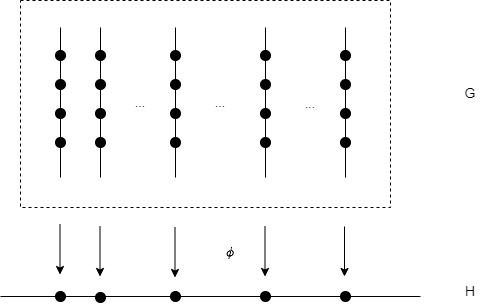
\includegraphics[scale=0.55]{images/2023-07-17-homomorphism.png}
\end{figure}

The classical example is to define $G$ as the numbers in $\mZ$ under the group operation addition $+$. The group $H$ is $\{0, 1\}$ under group operation addition $\mod 2$ (denoted as $\oplus$) and we define the map as $\phi(x) = x \mod 2$. This is a homomorphism, as can be easily checked: eg, we have $(1 + 4) \mod 2 = 5 \mod 2 = 1$ and $(1 \mod 2) \oplus (4 \mod 2) = 1 \oplus 0 = 1$.

There are two fibers: One is the set of elements in $G$ which are mapped by $\phi$ to $0$ in $H$ and this is the set of even numbers. The other fiber is the set of elements in $G$ which are mapped by $\phi$ to $1$ in $H$ and this is the set of odd numbers.

The group operation in $H$ provides a way to multiply two elements in the image of $\phi$. This suggests a natural multiplication of the \emph{fibers} lying above thw two points , thereby making the set of fibers into a group: If $X-a$ is the fiber above $a$ and $X_b$ is the fiber above $b$, then the product $X_a X_b$ is defined to be fiber $X_{ab}$ above the product $ab$; ie $X_a X_b = X_{ab}$. We can easily show that this defines a group and the group $G$ is partitioned into pieces (the fibers) and these pieces themselves have the structure of a group, called the \emph{quotient group} of $G$.

The \emph{kernel} is the set of elements in $G$ which map to the identity element of $H$; ie the fiber over the identity of $H$. More formally, we have the following definition.

\begin{definition}
If $\phi$ is a homomorphism from $G$ to $H$, then the kernel of $\phi$ is the set

\bee
\{g \in G | \phi(g) = e\}
\eee

where $e$ is the identity element of $H$.
\end{definition}

The kernel fulfills a couple of properties, we have $\phi(1_G) = 1H$, $\phi(g^{-1}) = \phi(g)^{-1}$, $\phi(g^n) = \phi(g)^n$ for all $n \in \mZ$ and finally the fact that the kernel is a subgroup of $G$.

\subsection{Quotient or Factor Groups}

With the kernel definition, we can define a \emph{quotient or factor group} as follows.

\begin{definition}
Let $\phi: G \rightarrow H$ be a homomorphism with kernel $K$. The quotient group or factor group, $G/K$,  is the group whose elements are the fibers of $\phi$ with group operation defined as follows: If $X$ denotes the fiber above $a$ and $Y$ denotes the fiber above $b$, then $X \cdot Y$ is defined as the fiber above $a \cdot b$.
\end{definition}

The notation emphasizes the fact that the kernel $K$ is a single element in the group $G/K$ and (we shall see) that the other elements of $G/K$ are the "translates" of $K$. Therefore we may think of $G/K$ as collapsing $G$ by $K$ and therefore also the name quotient group. In the definition above, the map $\phi$ enters the definition explicitely, but we can also define the multiplication of fibers in terms of \emph{representatives} from the fibers.

\begin{definition}
For any $N \leq G$ and any $g \in G$ let

\bee
gN = \{ gn | n \in N \}, \quad Ng = \{ ng | n \in N \}
\eee

called \emph{left coset} and \emph{right coset}, resepectively. Any element of a coset is a representative of the coset.

\end{definition}

We can use these cosets to provide another definition of $G/K$ as shown in the following theorem.

\begin{theorem}
Let $G$ be a group and $K$ be the kernel of some homomorphism from $G$ to another group. Then the set whose elements are the left cosets of $K$ in $G$ with operation defined by

\bee
uK \cdot vK = (uv)K
\eee

forms the group $G/K$. The operation is well-defined in the sense that if $u_1$ is any element in $uK$ and $v_1$ is any element in $vK$, then $u_1 v_1 \in uvK$ so that the multiplication does not depend on the choice of coset representatives $u_1, v_1$.

The theorem holds for right cosets as well.
\end{theorem}

Proof is omitted.

The relation between operations using coset elements / representatives and working with elements in $H$ is shown in the following Figure.

\begin{figure}[H]
\centering
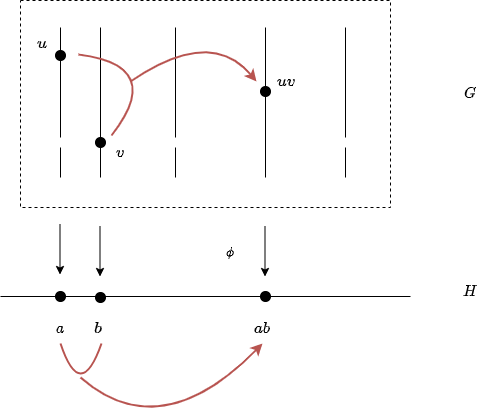
\includegraphics[scale=0.55]{images/2023-07-17-quotient_group.png}
\end{figure}

The important concept is that the multiplication is independent of the particular representative chosen; the product of two cosets $X$ and $Y$ is the coset $uvK$ containing the product $uv$ where $u$ and $v$ are \emph{any} representatives of the cosets $X$ and $Y$, respectively.

In the example from above, the kernel are the even numbers $u$ as $u \mod-2 = 0$. So the even numbers form a coset; the odd numbers another. The quotient group is then the set of even and odd numbers with group operation addition $\mod 2$. It does not matter which even or odd number we chose as representative.

\paragraph{Example.} Another example is $G = \mR^2$ with group operation vector addition. We define $\phi: \mR^2 \rightarrow R = \phi((x,y)) = x$; ie a projection of a point in the $x-y-$plane onto the $x-$axis. This is a homomorphism as

\bee
\phi((x_1, y_2) + (x_2, y_2)) = \phi((x_1 + x_2, y_1 + y_2)) = x_1 + x_2 = \phi((x_1, y_1)) + \phi((x_2, y_2))
\eee

For the kernel we obtain the set

\bee
\{ (x,y) | \phi((x,y)) = 0\} = \{ (x,y) | x = 0\}
\eee

which is the $y-$axis. The fiber of $\phi$ over $a \in mR$ is the line $x = a$. In a similar spirit, the cosets are the lines with $x = a$, we can chose any representative on these lines as $(a,y)$.

The group operation can be described by using the map $\phi$ as the sum of the line $x=a$ and the line $x=b$ is the line $x = a+b$ or in terms of cosets: The sum of the vertical line containing the point $(a, y_1)$ and the vertical line containing the point $(b, y_2)$ is the vertical line containing th point $(a+b,y)$. The representative does not matter; ie which point on the line we chose does not matter. \qed


By the previous theorem, if we are given a subgroup $K$ of a group $G$ which is the kernel od some homomorphism, we may define the quotient $G/K$ without recourse to the homomorphism by the multiplication $uK vK = uv K$. This raises the question whether we can define the quotient group $G/N$ for \emph{any} subgroup $N$ of $G$. The answer to this is no, as multiplication is in general not defined in this case. In fact, it is possible to define a quotient group iff $N$ is the kernel of some homomorphism.

We next show that the cosets of an arbitrary subgroup $G$ partition $G$.

\begin{theorem}
Let $N$ be any subgroup of a group $G$. The set of left cosets of $N$ in $G$ form a partition of $G$. In addition, $uN = vN$ iff $u$ and $v$ are representatives of the same coset.
\end{theorem}

Proof is omitted.

\begin{definition}
The element $gng^{-1}$ is called the conjugate of $n\in N$ by $g$. The set $gNg^{-1} = \{ gng^{-1} | n \in N \}$ is called the conjugate of $N$ by $g$. The element $g$ is said to normalize $N$ if $gNg^{-1} = N$. A subgroup $N$ of a group $G$ is called normal if every element of $G$ normalizes $N$; ie if $gNg^{-1} = N$ for all $g \in G$. If $N$ is a normal subgroup of $G$, we shall write $N \unlhd G$.
\end{definition}

With this definition in place, we can state the following theorem.

\begin{theorem}
Let $N$ be a subgroup of the group $G$. The following statements are equivalent:

\begin{itemize}
	\item $N \unlhd G$
	\item $N_G(N) = G$ where $N_g(N)$ is the normalizer in $G$ of $N$
	\item $gN = Ng$ for all $g \in G$
	\item Coset multiplication as defined above makes the set of left cosets into a group
	\item $gNg^{-1} \subseteq N$ for all $g \in G$.
\end{itemize}
\end{theorem}

And finally we have the fact that a normal subgroup is always the kernel of some homomorphism.

\begin{theorem}
A subgroup $N$ of a group $G$ is normal iff it is the kernel of some homomorphism.
\end{theorem}

Proof is omitted.

\subsection{Lagranges Theorem}

Lagranges theorem connects the group order of a group with its subgroup.

\begin{theorem}
If $G$ s a finite group and $H$ is a subgroup of $G$, then the order of $H$ divides the order of $G$ and the number of left cosets of $H$ in $G$ equals $|G| / |H|$.	
\end{theorem}

The proof relies on the fact that the cosets partition the group $G$.

The number of cosets of $H$ in $G$ is called the \emph{index} of $H$ in $G$ and is denoted by $|G:H|$.

\begin{theorem}
If $G$ is a finite group and $x \in G$, then the order of §x$ divides the order of $G$. In particaulr, $x^{|G|} = e$ for all $x \in G$.	
\end{theorem}

\begin{theorem}
If $G$ is a group of prime order $p$, then $G$ is cyclic and isomorphic to $\mZ_p$.
\end{theorem}


%%% Local Variables:
%%% mode: latex
%%% TeX-master: "journal"
%%% End:
